
\documentclass{article}
\usepackage{graphicx} % Required for inserting images
\usepackage{fancyhdr} % Required for header and footer configuration
\usepackage[a4paper, margin=2.5cm, left=1.5cm, right=1.5cm, bottom=4cm]{geometry} % Required for setting page margins
\usepackage[T1]{fontenc}
\usepackage[default,oldstyle,scale=1]{opensans} % Utilizzo del font Open Sans
\usepackage{lipsum}
\usepackage{makeidx}
\usepackage{booktabs}
\usepackage{tabularray}
\usepackage[colorlinks=true, linkcolor=black, urlcolor=blue, citecolor=blue]{hyperref}
\usepackage{tabularx}
\usepackage{makecell}
\usepackage{enumitem} % Pacchetto per la personalizzazione degli elenchi
\usepackage{booktabs}
\usepackage{subcaption}
\usepackage{pgfplots}
\usepgfplotslibrary{dateplot} % Per gestire gli assi con date

% Configure header and footer for the first page
\fancypagestyle{firstpage}{
    \fancyhf{} % Clear header and footer
    \renewcommand{\headrulewidth}{0pt} % Remove header rule line
    \lhead{} % Header on the left
    \chead{} % Header in the center
    \rhead{} % Header on the right
    \lfoot{} % Footer on the left
    \cfoot{\vspace{5pt}\\\hrulefill\\\vspace{10pt}\textbf{BeeLive}\\Gruppo 21} % Footer in the center
    \rfoot{\vspace{32.5pt}\\\thepage} % Footer on the right
}

% Configure header and footer for non-plain pages (second page onwards)
\fancypagestyle{nonplain}{
    \fancyhf{} % Clear header and footer
    \lhead{} % Header on the left
    \chead{} % Header in the center
    \rhead{\includegraphics[width=2cm]{Images/BeeLive-Logo.png}\\\vspace{2pt}} % Header on the right
    \lfoot{} % Footer on the left
    \cfoot{\vspace{5pt}\\\hrulefill\\\vspace{10pt}\textbf{BeeLive}\\Gruppo 21} % Footer in the center
    \rfoot{\vspace{32.5pt}\\\thepage} % Footer on the right
}

% Adjust vertical space between header and text                                    
\setlength{\headsep}{65pt} 
% Adjust vertical space between text and footer
\setlength{\footskip}{0pt} 

\title{\includegraphics[width=0.75\textwidth]{Images/BeeLive-Logo.png}\\\vspace{100pt}
\LARGE{\textbf{BeeLive\\Deliverable 4}}}
\author{Gruppo 21:\\
Cipriani Pietro, 226959\\
Orlando Dennis, 227688\\
Ziviani Elia, 228172}
\date{22 Aprile 2024}

\makeindex % Indica che vogliamo creare un indice

\begin{document}

\maketitle
\thispagestyle{firstpage} % Apply firstpage style to the first page
\clearpage

\pagestyle{nonplain} % Apply non-plain style to subsequent pages

\renewcommand{\contentsname}{Indice}
\tableofcontents

\clearpage

\section{Revisione}



\section{Introduzione}

\subsection{Componenti del gruppo}
\begin{itemize}
    \item Cipriani Pietro, matricola 226959, \lbrack\href{https://github.com/pietrocipriani}{github profile}\rbrack
    \item Orlando Dennis, matricola 227688, \lbrack\href{https://github.com/dennisorlando}{github profile}\rbrack
    \item Ziviani Elia, matricola 228172, \lbrack\href{https://github.com/ELI20ZIVI}{github profile}\rbrack
\end{itemize}

\subsection{Scopo del progetto}

Lo scopo del progetto 'BeeLive' è quello di risolvere il problema riguardante la difficoltà nel reperire informazioni riguardanti gli eventi che influenzano la viabilità all'interno del Comune di Trento. Prevediamo un sistema informativo, dedicato agli utenti cittadini, che mostri visualmente le variazioni della viabilità in città, informando gli stessi di eventuali modifiche che potrebbero colpirli direttamente.

\subsection{Link utili}
Il primo link fornito è quello della repository github. La repository è stata creata appena il corso è cominciato, infatti inizialmente è risultata utile al fine di scrivere in modo collaborativo i primi deliverable.\\
E' stato deciso di integrare in questa repository anche le fasi di sprint in quanto come team riteniamo utile la possibilità di accedere alla documentazione redatta nei primi due deliverable.\\
La repository è accessibile al seguente link: \href{https://github.com/ELI20ZIVI/BeeLive/}{Repository GitHub}\\ \\
Il secondo link fornito è quello di Apiary. Apiary è uno strumento che permette di creare e documentare in modo molto accurato e approfontido le API utilizzate nel progetto.\\
Il link di Apiary è il seguente: \href{https://beelive.docs.apiary.io/#}{Link Apiary}\\

\clearpage

\section{Sezione generale}

\subsection{Strategia di Branching}

Per lo sviluppo dell'applicativo è stato evitato l'approccio "Master only": nonostante la piccola dimensione del team, la creazione ed utilizzo di un unico branch principale, \textit{main}, avrebbe comunque causato problemi di collaborazione e conflitti nel momento in cui avremmo lavorato contemporaneamente a stesse sezioni del progetto.\\

\noindent
Per aumentare la modulabilità e la scalabilità del progetto, abbiamo infatti adottato la strategia di branching prevedente la creazione di un 'branch' separato per ogni specifica feature del progetto, con un branch \textit{develop} intermedio.\\

\noindent
L'integrazione di una feature specifica avviene attraverso il merging del branch di quest'ultima nel precedentemente citato \textit{develop}; tale operazione è ammessa solamente da un diverso componente del gruppo, il cui compito sarà quello di assicurarsi che il modulo rispetti tutti i punti della "Definition of Done" definita dal team. \\

\noindent
Dato il branch \textit{develop}, definito come ambiente di lavoro in cui i membri del team lavorano e accumulano modifiche, una volta che ne sono accumulate abbastanza (e giudicato lo stato del progetto per intero come 'stabile' e 'shippable') verrà effettuato il merge di questa branch nel principale \texttt{main}, come operazione di 'release'. \\

\noindent
Tramite questo approccio puntiamo ad incrementare la collaborazione tra i membri del team, ridurre i conflitti e le inconsistenze nel codice, facilitare la gestione delle diverse attività in corso e mantenere inoltre una mappatura di tutte le diverse modifiche e progressi del progetto, mantenendo ben strutturata la storia del codice.\\

Segue una lista dei branch utilizzati per lo sviluppo del progetto; da notare che molte di queste branches sono state eliminate una volta integrate in \texttt{develop}, per cui su github potrebbero non apparire.



\clearpage

\subsection{Product Backlog}
Nella pagina seguente vi è riportato il product backlog che abbiamo sviluppato per questo progetto. E' possibile notare una linea di demarcazione che limita inferiormente le entries selezionate per il primo sprint.

\begin{table}[!ht]
    \centering
    \renewcommand{\arraystretch}{1.3} % Imposta lo spazio verticale delle righe
    \begin{tabularx}{\textwidth}{| r | X | r | r |}
        \Xhline{2pt}
        \makecell{\textbf{Nome}} & \makecell{\textbf{User story}} & \makecell{\textbf{Priorità}} & \makecell{\textbf{Stima}} \\
        \Xhline{2pt}
        \makecell{Visualizzazione\\eventi in città} & \makecell{Da utente, voglio visualizzare la lista degli eventi in città} & \makecell{200} & \makecell{8}\\
        \hline
        \makecell{Aggiunta eventi\\da utente\\autorizzato} & \makecell{Da utente autorizzato, devo essere in grado di aggiungere degli eventi\\in modo da comunicare la loro presenza agli utenti} & \makecell{190} & \makecell{8}\\
        \hline
        \makecell{Registrazione e\\accesso all'\\app mobile} & \makecell{Da utente, voglio avere la possibilità di accedere ad una\\visualizzazione e descrizione più dettagliata di un evento in modo da\\conoscere meglio le specifiche di tale evento} & \makecell{180} & \makecell{8}\\
        \hline
        \makecell{Visualizzazione\\criticità\\su mappa} & \makecell{Da utente, voglio visualizzare su una cartina le zone colpite dai diversi\\eventi, in modo da capire visivamente se in una zona che mi\\interessa vi è un evento attivo} & \makecell{170} & \makecell{6}\\
        \hline
        \makecell{Accesso alle\\criticità e ai\\loro dettagli} & \makecell{Da utente, voglio essere in grado di visualizzare la lista\\delle criticità presenti in città} & \makecell{160} & \makecell{8}\\
        \Xhline{2pt}
        \makecell{Impostazione\\categorie\\d'interesse\\per gli eventi} & \makecell{Da utente, voglio essere in grado di impostare le categorie di eventi\\alle quali io sono interessato, in modo che la lista di eventi visibile\\dall'applicazione contenga solamente gli eventi che mi interessano,\\e in modo che io non venga notificato di alcun evento\\che io non ritenga appartenere ad una categoria interessante} & \makecell{100} & \makecell{5}\\
        \hline
        \makecell{Impostazione\\zone\\d'interesse} & \makecell{Da utente, voglio essere in grado di impostare delle zone di interesse,\\in modo che io venga notificato di qualsiasi evento che insorga\\in una di queste zone} & \makecell{90} & \makecell{7}\\
        \hline
        \makecell{Visualizzazione\\eventi\\di competenza} & \makecell{Da utente autorizzato, devo essere in grado di visualizzare gli eventi\\di mia competenza, in modo da sapere quali eventi sono stati creati e\\monitorare il loro stato} & \makecell{80} & \makecell{5}\\
        \hline
        \makecell{Modifica\\eventi} & \makecell{Da utente autorizzato, devo essere in grado di modificare degli eventi\\in modo da evitare errori comunicativi} & \makecell{75} & \makecell{2}\\
        \hline
        \makecell{Accesso\\account\\utente} & \makecell{Da utente registrato, voglio essere in grado di poter accedere al\\mio account in modo da poter riottenere le aree di interesse e\\le impostazioni che ho precedentemente salvato} & \makecell{70} & \makecell{3}\\
        \hline
        \makecell{Visualizzazione\\eventi\\di categorie\\di interesse} & \makecell{Da utente, voglio essere in grado di visualizzare solo\\eventi di categorie di interesse} & \makecell{60} & \makecell{3}\\
        \hline
        \makecell{Selezione\\percorso} & \makecell{Da utente, voglio essere in grado di selezionare un percorso a partire\\da dei waypoint, per impostare dei percorsi di interesse} & \makecell{40} & \makecell{2}\\
        \hline
        \makecell{Eliminazione\\eventi} & \makecell{Da utente autorizzato, devo essere in grado di eliminare degli eventi} & \makecell{40} & \makecell{2}\\
        \hline
    \end{tabularx}
    \caption{Product backlog}
\end{table}

\clearpage

\subsection{Definition of "Done"}
La seguente 'Definition of Done' è basata su una valutazione collettiva che ha preso in considerazione  diversi fattori riguardanti la qualità del lavoro, non ignorando però la fattibilità e la realizzabilità di questi.\\
I criteri inclusi nella nostra 'Definition of Done' definita per il progetto sono i seguenti:
\begin{itemize}
	\item \textbf{Funzionalità}: le funzionalità che il codice implementa devono soddisfare appieno l'usecase / gli usecase associati al codice.
    \item \textbf{Codice}: Il codice deve essere revisionato e la sua correttezza / adeguatezza approvata da almeno un altro membro del team.
    \item \textbf{Test}: Il codice deve essere adeguatamente coperto da test unitari, di integrazione e funzionali, che devono essere scritti e superati con successo. Un adeguato numero di questi test deve essere scritto da membri diversi.
    \item \textbf{Documentazione}: Il codice e le funzionalità implementate devono essere adeguatamente documentati. Questo giudizio di adeguatezza deve essere dato da almeno un altro membro del team.
    \item \textbf{Build e Deployment}: Il codice deve integrarsi con successo nella build principale e la sua inclusione nella build principale non deve assolutamente far fallire dei test, nel caso in cui quest'ultimi venivano correttamente superati priva dell'inclusione.
    \item \textbf{Performance}: le funzionalità e il codice introdotti non devono causare visibili degradi alle performance di nessun elemento del progetto.
    \item \textbf{Conformità}: Il prodotto deve essere conforme alle normative legali e agli standard di sicurezza e qualità specifici del settore.
\end{itemize}

\clearpage

\section{Sezione Sprint \#1}

\subsection{Goal dello sprint}
Lo scopo di questo primo sprint è stato quello di creare un prototipo funzionante dell'applicazione, che presenti le funzionalità core del nostro progetto e che quindi includa queste funzionalità:
\begin{enumerate}
\item Possibilità da parte di un utente autorizzato di aggiungere eventi al sistema
\item Possibilità da parte degli utenti di visualizzare gli eventi aggiunti
\end{enumerate}
È stato dunque necessario lavorare, oltre al 'backend', anche allo sviluppo sia dell'applicativo mobile dedicato ad utenti comuni che all'applicativo desktop, dedicato agli utenti autorizzati.

Scendendo più in dettaglio, le funzionalità che abbiamo deciso di includere nello sprint sono, per quanto riguarda la parte mobile, la visualizzazione degli eventi disponibili e dei loro relativi dettagli, anche includendo la visualizzazione su mappa.\\
E' stato inoltre inserita, anche se con bassa priorità, la funzionalità riguardante la possibilità di effettuare l'autenticazione (da parte degli utenti comuni) per poter salvare le proprie impostazioni e preferenze sul database.\\
Per quanto riguarda la parte desktop, ci siamo limitati a rendere possibile l'aggiunta degli eventi al sistema, rimandando l'autenticazione degli utenti autorizzati a sprint successivi.

\subsection{Sprint Planning}
E' riportato il product backlog per ogni user story trattata in questo primo sprint, con tutte le informazioni relative ai task da completare, a chi sono assegnati e la loro priorità.\\
\subsubsection{}
\textbf{User story}: 

\textbf{Product backlog}
\begin{table}[htbp]
    \centering
    \renewcommand{\arraystretch}{1.3} % Imposta lo spazio verticale delle righe
    \begin{tabularx}{\textwidth}{| X | r | r | r | r |}
        \Xhline{2pt}
        \makecell{\textbf{Nome}} & \makecell{\textbf{User story}} & \makecell{\textbf{Cosa fare}} & \makecell{\textbf{Assegnazione}} & \makecell{\textbf{Stima}} \\
        \Xhline{2pt}
        \makecell{} & \makecell{} & \makecell{} & \makecell{} & \makecell{} \\
        \hline
    \end{tabularx}
    \caption{Product backlog user story 1}
\end{table}


\subsection{Burndown chart}
Il burndown chart è uno strumento utilizzato per monitorare il progresso di un progetto.\\
Giorno per giorno si può visualizzare l'andamento dei lavori e capire se si sta procedendo secondo i piani o se ci sono ritardi.\\

\begin{figure}[htbp]
    \centering
    \begin{tikzpicture}
        \begin{axis}[
            width=12cm, height=8cm, % Dimensioni del grafico
            date coordinates in=x,
            xlabel={Date},
            ylabel={Tasks Remaining},
            xticklabel={\day-\month},
            grid=major,
            legend pos=north east,
        ]
        \addplot[
            color=blue,
            mark=square*,
            thick
        ] table [col sep=comma, x=date, y=planned] {
            date, planned
            2024-05-01, 122
            2024-05-16, 0
        };
        \addlegendentry{Planned}

        \addplot[
            color=red,
            mark=triangle*,
            thick
        ] table [col sep=comma, x=date, y=actual] {
            date, actual
            2024-05-01, 122
            2024-05-02, 117
            2024-05-03, 115
            2024-05-04, 113
            2024-05-05, 109
            2024-05-06, 96
            2024-05-07, 83
            2024-05-08, 79
            2024-05-09, 76
            2024-05-10, 74
            2024-05-11, 65
            2024-05-12, 60
            2024-05-13, 48
            2024-05-14, 42
            2024-05-15, 42
            2024-05-16, 42
        };
        \addlegendentry{Actual}
        \end{axis}
    \end{tikzpicture}
    \caption{Burndown Chart}
    \label{fig:burndown}
\end{figure}

\clearpage

\subsection{Test cases}
\subsubsection{Test cases per il modulo \texttt{public\_server}}
Il modulo \texttt{public\_server} è il modulo che si occupa di gestire le richieste provenienti dall'applicativo mobile.\\
Infatti ha il compito di gestire tutte le richieste provenienti dagli applicativi mobile installati sui dispositivi, andando quindi a reperire dal database tutti gli eventi che sono richiesti nella richiesta stessa.\\

\begin{itemize}
    \item Test case per la richiesta di tutti gli eventi:
\end{itemize}

\begin{table}[htbp]
    \centering
    \renewcommand{\arraystretch}{1.3} % Imposta lo spazio verticale delle righe
    \begin{tabularx}{\textwidth}{| r | X | X | X | X | X | X |}
        \Xhline{2pt}
        \makecell{\textbf{No.}} & \makecell{\textbf{Descrizione}} & \makecell{\textbf{Dati}} & \makecell{\textbf{Precondizioni}} & \makecell{\textbf{Risultati attesi}} & \makecell{\textbf{Note}} \\
        \Xhline{2pt}
         &  &  &  &  &  \\
        \hline
    \end{tabularx}
\end{table}

\subsection{Deploy}
Il deployment del progetto attuale è effettuabile attraverso 3 container "Docker", creati da noi, connessi tramite docker-compose.
In particolare, in \texttt{BeeLive/Products/Docker} vi è un file "docker-compose.yml" che, intuitivamente, va usato con il tool "docker-compose".\\
Questo docker-compose si occupa di costruire e avviare tutti i container, costruiti da noi, contenenti le diverse componenti del "backend". \\\\
Tale deployment è già utilizzabile attraverso le due applicazioni (mobile e desktop) che abbiamo creato, sebbene gli indirizzi IP siano da modificare.
\\
Documentazione ulteriore verrà a seguire nel prossimo deliverable, in quanto le configurazioni sono ancora volatili e soggette a possibili cambiamenti.\\
\\
Questi container sono attualmente in esecuzione su un nostro server di testing con ip statico \textit{93.49.96.13}, per cui se i lettori vogliono possono provare già a testare gli endpoint creati. 


\subsection{Sprint review}

\subsection{Product backlog refinement}

\subsection{Sprint retrospective}

\end{document}
